\documentclass[11pt]{article}
\usepackage[T1]{fontenc}\usepackage{lmodern,amsmath,amssymb,graphicx,geometry,microtype,caption}
\usepackage[hidelinks]{hyperref}\geometry{letterpaper,margin=1in}
\pagestyle{empty}\setlength{\emergencystretch}{2em}
\renewcommand{\thefigure}{S\arabic{figure}}\setcounter{figure}{7}
\begin{document}
\begin{figure}[!ht]\centering
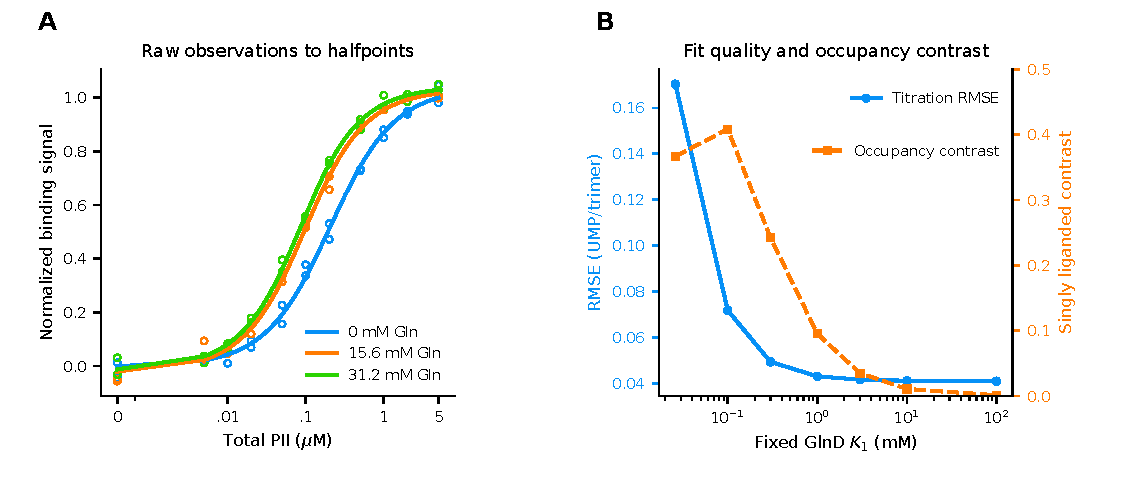
\includegraphics[width=\textwidth]{figure_inputs/raw_and_profile.pdf}
\caption{\textbf{Raw-assay fits and GlnD profiles retain different diagnostic roles.} (A) One simulated three-condition GlnE titration, with two readings at eleven doses. Lines show finite-depletion fits with separate background and gain for each glutamine condition. This synthetic example uses $\alpha_1=0.25$ and $K_G=15.6$ mM; complete raw observations and fitted parameters are supplied in S1 Data. (B) GlnD fixed-$K_1$ profiles retaining two endpoint specificity ratios while releasing the fixed-capacity, intermediate-state and transported 0.080 mM UR half-range restrictions. Titration RMSE improves as the available singly liganded occupancy contrast shrinks. These profiles are cross-assay stress hypotheses, not confidence intervals or measured binding affinities.}
\end{figure}
\end{document}
